\documentclass[13pt]{beamer}

%% Packages

\usepackage{mathtools, amsthm}
\usepackage{exercise-sheet}
\usepackage{global-macros}
\usepackage{tikz}
\usetikzlibrary{positioning}
\usepackage[
    backend=biber,
    style=alphabetic,
    sorting=ynt
]{biblatex}
\usepackage{csquotes}
\usepackage{hyperref}

%% Environments

\theoremstyle{plain} % default
\newtheorem{teo}{Teorema}[section]
\newtheorem{lem}{Lema}[section]
\newtheorem{prop}{Proposição}[section]
\newtheorem{cor}[teo]{Corolário}
\newtheorem*{axiom}{Axioma}

\newtheorem*{TAU}{Teorema da Aproximação Universal}
\newtheorem*{Riesz}{Teorema da Representação de Riesz}

\theoremstyle{definition}
\newtheorem{defn}{Definição}[section]
\newtheorem{conj}{Conjectura}[section]
\newtheorem{exmp}{Exemplo}[section]
\newtheorem{rem}{Observação}[section]

\theoremstyle{remark}
\newtheorem*{note}{Nota}
\newtheorem{case}{Caso}


% Macros

\renewcommand{\vec}[1]{\mathbf{#1}}
\renewcommand{\Re}{\text{Re}}

\newcommand{\K}{\mathbb{K}}
\newcommand{\I}{\mathbb{I}}
\newcommand{\uat}{\textbf{TAU}}

\DeclarePairedDelimiter{\dotprod}{\langle}{\rangle}

\DeclareMathOperator{\rk}{rk}
\DeclareMathOperator{\intt}{int}
\DeclareMathOperator{\diam}{diam}
\DeclareMathOperator{\rref}{rref}
\DeclareMathOperator{\vspan}{span}
\DeclareMathOperator{\proj}{proj}
\DeclareMathOperator{\lin}{Lin}
\DeclareMathOperator{\supp}{supp}

%% Numbering

\numberwithin{equation}{section}

\usepackage{global-macros}

\begin{comment}
    Estrutura:
     - Slide inicial
        -- Falar por alto a ideia do Teorema.
     - Explicar o que é uma rede neural
        -- Blá blá sobre inspiração nos neurônios do cérebro
        -- Imagem clássica da feedforward network
        % -- Link para os vídeos do 3b1b
     - Apliações de redes neurais
        -- Citar algumas aplicações bem sucedidas (links para wikipédia)
        -- Reforçar a importância do TAU

     - Mostrar artigo do Cybenko
        -- Enunciar Teorema igual na introdução do relatório
        -- Referência do Artigo
        -- Print da demonstração
     - Interludio: começar mais de baixo
        -- Apresentar Weirstrass e Hilbert
        -- Explicar por que estudar esses resultados antes
            --- TAU muito avançado para o que eu sabia
            --- Curso de medida ainda começando
            --- Interessante estudar aproximadores em contextos
                mais simples
     - Aproximação de Weierstrass
       -- Contexto mais simples
       -- Enunciar Teorema
       -- Já introduzir norma infinito e notação
       -- Dar ideia da demonstração, usando polinômios de bernstein
     - Ilustrar Weierstrass
       -- Mostrar polinômios de Bernstein aproximando uma função ****
     - Hilbert
       -- Introduzir problema, falar brevemente sobre como ele foi
          formulado inicialmente
       -- Falar um pouco da história do resultado
       -- Comentar sobre diferenças com relação aos teoremas anteriores
           --- Aproximação vs Representação Exata
     - Tentar dar uma ideia da demonstração do 13 de Hilbert
     - Fim do interlúdio: Volta ao TAU
       -- Fazer diagrama ilustrando resultados necessários para mostrar o TAU
     - Pincelada da Prova
       -- Fornecer principais passos da demonstração em tópicos, mostrando onde
          cada Teorema é Utilizado
       -- Falar sobre lema que contém boa parte da demonstração (sigmoide é
          discriminatória)
     - Hahn Banach
       -- Enunciar Teorema, falar um pouco da importância dele
       -- Falar sobre resultados necessários para prová-lo
       -- Ilustrar de alguma forma o Teorema
     - Enunciar o corolário que realmente vai ser utilizado na prova do TAU
       -- Dar ideia da demonstração
     - Representação de Riesz
       -- Falar sobre diferentes versões do Teorema
       --- Em Análise Funcional (Espaços de Hilbert)
           --- Em Teorema da Medida (Espaços L_p)
           --- No contexto do TAU
       -- Enunciar Teorema que o Cybenko usa, falar que tava fora da minha alçada
       -- Enunciar versão mais simples, dar ideia da demonstração
     - Reapresentar demonstração do TAU
       -- Falar do Lema
     - Enunciar lema e dar ideia da demonstração
     - Ilustrar TAU com um exemplo mais de boa, por exemplo alguma função real
       em R² ****
     - Problemas do TAU
       -- Falar de bounds para o número de neurônios na camada intermediária
       -- Problema de achar a rede que aproxima a função (SGD)
     - Generalizações
        -- Comentar sobre resultados relativos a aproximação de derivadas
     - Falar de próximos passos da IC
       -- DGM
     - Link para Repositório do Github
     - Agradecimentos
       -- Yuri, CNPq
\end{comment}

%% TODO: Colocar nome do Yuri no primeiro slide
%%       Arrumar algum lugar pra falar da bolsa do PICME
%%       Arrumar Repositório da IC
%%       Precisa de referenciar imagens? tipo a da rede com várias camadas

\title[Teorema da Aproximação Universal]{Sobre O Teorema da Aproximação Universal}
\author[C. Lins]{{Caio Lins}}
%%     {\and} 
%%     {\textit{Orientador}} 
%%     {Yuri Saporito}}
\institute[EMAp]{FGV - EMAp}
\date[EMAp 2021]{Outubro 2021}
\logo{\includegraphics[height=0.8cm]{../figuras/fgv_logo.png}}


\begin{document}

\maketitle

%%%%%%%%%%%%%%%%%%%%%%%%%%%%%%%%%%%%%%%%%%%%%%%%%%%%%%%%%%%
%%%%%%%%%%%%%%% Intro a Redes Neurais %%%%%%%%%%%%%%%%%%%%%
%%%%%%%%%%%%%%%%%%%%%%%%%%%%%%%%%%%%%%%%%%%%%%%%%%%%%%%%%%%

\begin{frame}{Overview de Redes Neurais}{O que são redes neurais?}
    \begin{itemize}
        \item Redes neurais são algoritmos que espelham o funcionamento do cérebro humano.
            É organizada em camadas de ``neurônios''.
    \end{itemize}
    \begin{figure}
        \begin{center}
            % !TeX root = ../main.tex

\tikzset{%
  every neuron/.style={
    circle,
    draw,
    minimum size=1cm
  },
  neuron missing/.style={
    draw=none, 
    scale=3,
    text height=0.3cm,
    execute at begin node=\color{black}$\vdots$
  },
}

\vspace{.6cm}

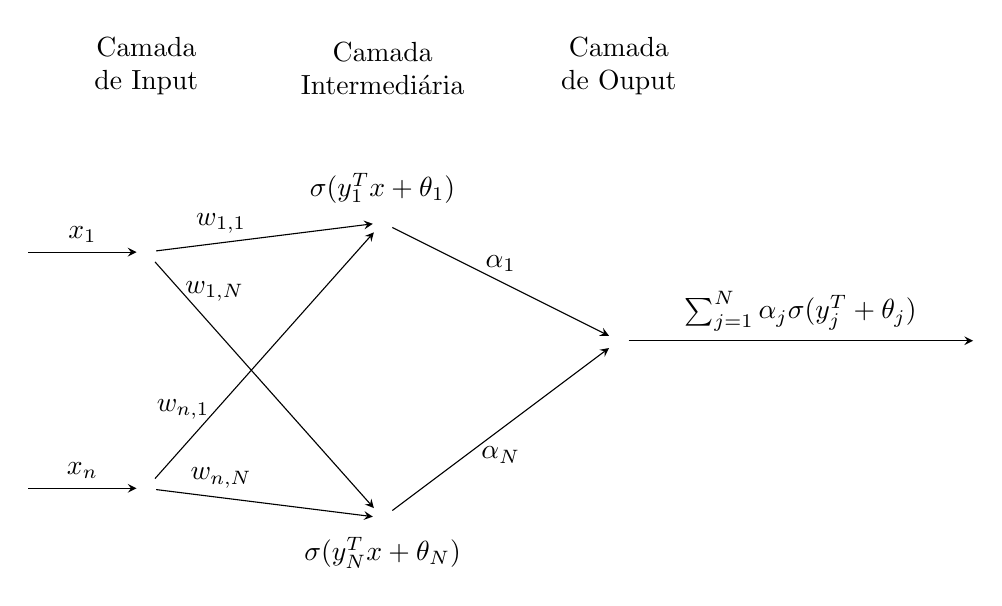
\begin{tikzpicture}[x=1.5cm, y=1.5cm, yshift=-1, >=stealth]

\foreach \m/\l [count=\y] in {1,missing,2}
  \node [every neuron/.try, neuron \m/.try] (input-\m) at (0,1.75-\y) {};

\foreach \m [count=\y] in {1,missing,2}
  \node [every neuron/.try, neuron \m/.try ] (hidden-\m) at (2,2.25-\y*1.25) {};

\foreach \m [count=\y] in {1}
  \node [every neuron/.try, neuron \m/.try ] (output-\m) at (4,1-\y) {};

\foreach \l [count=\i] in {1,n}
  \draw [<-] (input-\i) -- ++(-1,0)
    node [above, midway] {$x_\l$};

%% \foreach \l [count=\i] in {1,n}
%%   \node [above] at (hidden-\i.north) {$H_\l$};
\node [above] at (hidden-1.north) {\( \sigma (y_{ 1 }^{ T }x + \theta_{ 1 }) \)};
\node [below] at (hidden-2.south) {\( \sigma (y_{ N }^{ T }x + \theta_{ N }) \)};

\foreach \l [count=\i] in {1}
  \draw [->] (output-\i) -- ++(3,0)
    node [above, midway] {\( \sum_{ j=1 }^{ N } \alpha_{ j } \sigma (y_{ j }^{ T } + \theta_{ j }) \)};

%% \foreach \i in {1,...,2}
%%   \foreach \j in {1,...,2}
%%     \draw [->] (input-\i) -- (hidden-\j)
%%         node [above,pos=.2] {\( y_{ 1 }^{ (1) } \)};
\draw [->] (input-1) -- (hidden-1)
    node [above, pos=.3] {\( w_{ 1,1 } \)};
\draw [->] (input-2) -- (hidden-1)
    node [above, pos=.2, xshift=-2mm] {\( w_{ n,1 } \)};
\draw [->] (input-1) -- (hidden-2)
    node [above, pos=.2,xshift=2mm] {\( w_{ 1,N } \)};
\draw [->] (input-2) -- (hidden-2)
    node [above, pos=.3] {\( w_{ n,N } \)};

%% \foreach \i in {1,...,2}
%%   \foreach \j in {1}
%%     \draw [->] (hidden-\i) -- (output-\j);
\draw [->] (hidden-1) -- (output-1)
    node [above, midway] {\( \alpha_{ 1 } \)};
\draw [->] (hidden-2) -- (output-1)
    node [below, midway, yshift=-1mm] {\( \alpha_{ N } \)};

\foreach \l [count=\x from 0] in {de Input, Intermediária, de Ouput}
  \node [align=center, above] at (\x*2,2) {Camada \\ \l};

\end{tikzpicture}
        \end{center}
    \end{figure}
\end{frame}

\begin{frame}{Overview de Redes Neurais}{O que são redes neurais?}
    \begin{itemize}
        \item Input: \( \bfx = ( x_{ 1 }, \dots, x_{ n } ) \in \R^{ n } \).
        \item Pesos (\emph{weights}): \( \bfw_{ j } = ( w_{ 1, j }, \dots, w_{ N, j } ) \in \R^{ n }, j = 1, \dots, N \).
        \item Viéses (\emph{biases}): \( \theta_{ j } \in \R , j = 1, \dots, N\).
        \item Função de ativação: \( \sigma : \R \to \R \).
    \end{itemize}
    \begin{center}
        % !TeX root = ../main.tex

\tikzset{%
  every neuron/.style={
    circle,
    draw,
    minimum size=1cm
  },
  neuron missing/.style={
    draw=none, 
    scale=3,
    text height=0.3cm,
    execute at begin node=\color{black}$\vdots$
  },
}

\vspace{.6cm}

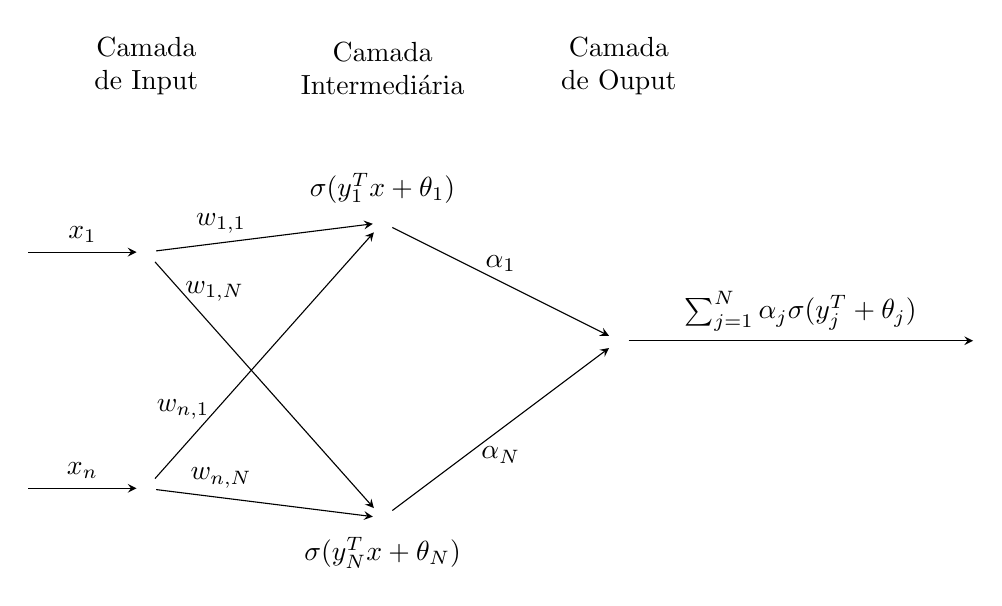
\begin{tikzpicture}[x=1.5cm, y=1.5cm, yshift=-1, >=stealth]

\foreach \m/\l [count=\y] in {1,missing,2}
  \node [every neuron/.try, neuron \m/.try] (input-\m) at (0,1.75-\y) {};

\foreach \m [count=\y] in {1,missing,2}
  \node [every neuron/.try, neuron \m/.try ] (hidden-\m) at (2,2.25-\y*1.25) {};

\foreach \m [count=\y] in {1}
  \node [every neuron/.try, neuron \m/.try ] (output-\m) at (4,1-\y) {};

\foreach \l [count=\i] in {1,n}
  \draw [<-] (input-\i) -- ++(-1,0)
    node [above, midway] {$x_\l$};

%% \foreach \l [count=\i] in {1,n}
%%   \node [above] at (hidden-\i.north) {$H_\l$};
\node [above] at (hidden-1.north) {\( \sigma (y_{ 1 }^{ T }x + \theta_{ 1 }) \)};
\node [below] at (hidden-2.south) {\( \sigma (y_{ N }^{ T }x + \theta_{ N }) \)};

\foreach \l [count=\i] in {1}
  \draw [->] (output-\i) -- ++(3,0)
    node [above, midway] {\( \sum_{ j=1 }^{ N } \alpha_{ j } \sigma (y_{ j }^{ T } + \theta_{ j }) \)};

%% \foreach \i in {1,...,2}
%%   \foreach \j in {1,...,2}
%%     \draw [->] (input-\i) -- (hidden-\j)
%%         node [above,pos=.2] {\( y_{ 1 }^{ (1) } \)};
\draw [->] (input-1) -- (hidden-1)
    node [above, pos=.3] {\( w_{ 1,1 } \)};
\draw [->] (input-2) -- (hidden-1)
    node [above, pos=.2, xshift=-2mm] {\( w_{ n,1 } \)};
\draw [->] (input-1) -- (hidden-2)
    node [above, pos=.2,xshift=2mm] {\( w_{ 1,N } \)};
\draw [->] (input-2) -- (hidden-2)
    node [above, pos=.3] {\( w_{ n,N } \)};

%% \foreach \i in {1,...,2}
%%   \foreach \j in {1}
%%     \draw [->] (hidden-\i) -- (output-\j);
\draw [->] (hidden-1) -- (output-1)
    node [above, midway] {\( \alpha_{ 1 } \)};
\draw [->] (hidden-2) -- (output-1)
    node [below, midway, yshift=-1mm] {\( \alpha_{ N } \)};

\foreach \l [count=\x from 0] in {de Input, Intermediária, de Ouput}
  \node [align=center, above] at (\x*2,2) {Camada \\ \l};

\end{tikzpicture}
    \end{center}
\end{frame}

\begin{frame}{Overview de Redes Neurais}{O que são redes neurais?}
    \vspace{2pt}
    O \( j \)-ésimo neurônio da camada oculta computa a soma
    \begin{equation*}
        \bfw_{ j }^{ \transpose } \bfx + \theta_{ j } = w_{ 1, j }x_{ 1 } + w_{ 2,j } x_{ 2 } + \cdots + w_{ n, j } x_{ n } + \theta_{ j }
    \end{equation*}
    e passa o resultado pela ativação \( \sigma : \R \to \R \), que é \emph{não linear}.
    \begin{center}
        % !TeX root = ../main.tex

\tikzset{%
  every neuron/.style={
    circle,
    draw,
    minimum size=1cm
  },
  neuron missing/.style={
    draw=none, 
    scale=3,
    text height=0.3cm,
    execute at begin node=\color{black}$\vdots$
  },
}

\vspace{.6cm}

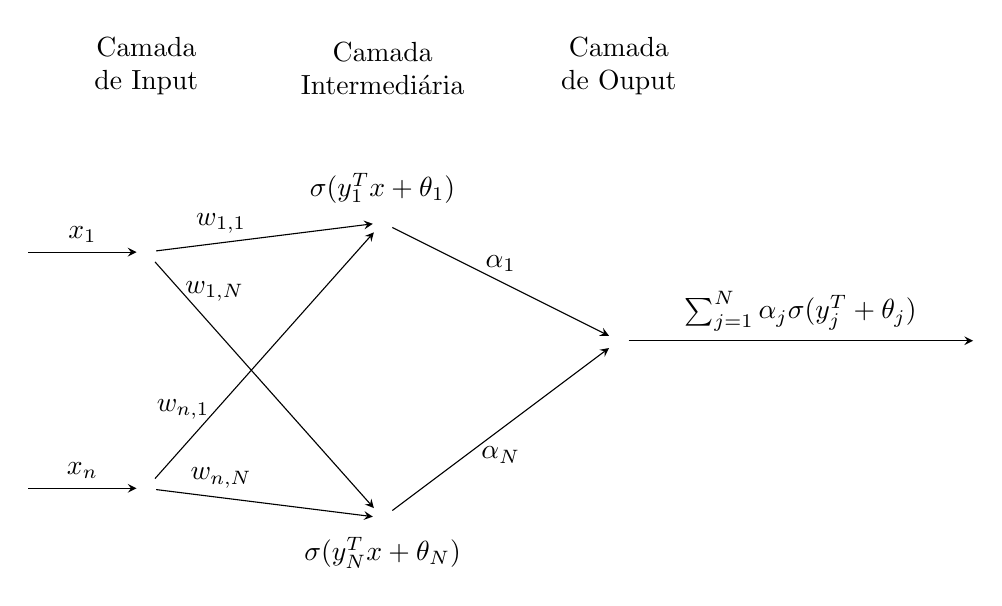
\begin{tikzpicture}[x=1.5cm, y=1.5cm, yshift=-1, >=stealth]

\foreach \m/\l [count=\y] in {1,missing,2}
  \node [every neuron/.try, neuron \m/.try] (input-\m) at (0,1.75-\y) {};

\foreach \m [count=\y] in {1,missing,2}
  \node [every neuron/.try, neuron \m/.try ] (hidden-\m) at (2,2.25-\y*1.25) {};

\foreach \m [count=\y] in {1}
  \node [every neuron/.try, neuron \m/.try ] (output-\m) at (4,1-\y) {};

\foreach \l [count=\i] in {1,n}
  \draw [<-] (input-\i) -- ++(-1,0)
    node [above, midway] {$x_\l$};

%% \foreach \l [count=\i] in {1,n}
%%   \node [above] at (hidden-\i.north) {$H_\l$};
\node [above] at (hidden-1.north) {\( \sigma (y_{ 1 }^{ T }x + \theta_{ 1 }) \)};
\node [below] at (hidden-2.south) {\( \sigma (y_{ N }^{ T }x + \theta_{ N }) \)};

\foreach \l [count=\i] in {1}
  \draw [->] (output-\i) -- ++(3,0)
    node [above, midway] {\( \sum_{ j=1 }^{ N } \alpha_{ j } \sigma (y_{ j }^{ T } + \theta_{ j }) \)};

%% \foreach \i in {1,...,2}
%%   \foreach \j in {1,...,2}
%%     \draw [->] (input-\i) -- (hidden-\j)
%%         node [above,pos=.2] {\( y_{ 1 }^{ (1) } \)};
\draw [->] (input-1) -- (hidden-1)
    node [above, pos=.3] {\( w_{ 1,1 } \)};
\draw [->] (input-2) -- (hidden-1)
    node [above, pos=.2, xshift=-2mm] {\( w_{ n,1 } \)};
\draw [->] (input-1) -- (hidden-2)
    node [above, pos=.2,xshift=2mm] {\( w_{ 1,N } \)};
\draw [->] (input-2) -- (hidden-2)
    node [above, pos=.3] {\( w_{ n,N } \)};

%% \foreach \i in {1,...,2}
%%   \foreach \j in {1}
%%     \draw [->] (hidden-\i) -- (output-\j);
\draw [->] (hidden-1) -- (output-1)
    node [above, midway] {\( \alpha_{ 1 } \)};
\draw [->] (hidden-2) -- (output-1)
    node [below, midway, yshift=-1mm] {\( \alpha_{ N } \)};

\foreach \l [count=\x from 0] in {de Input, Intermediária, de Ouput}
  \node [align=center, above] at (\x*2,2) {Camada \\ \l};

\end{tikzpicture}
    \end{center}
\end{frame}

\begin{frame}{Overview de Redes Neurais}{O que são redes neurais?}
    \vspace{2pt}
    Existem várias funções de ativação possíveis, mas tenham em mente a \emph{função logística}, que também será chamada de \emph{sigmoide}:
    \begin{equation*}
        \sigma ( x ) = \frac{ 1 }{ 1 + e^{ -x } }
    .\end{equation*}
    \begin{center}
        \begin{tikzpicture}[scale=1]
    \begin{axis}[
        axis x line=middle,
        axis y line=middle,
        yscale=.6,
        ylabel=\( \sigma ( x ) \),
        ytick={1},
        yticklabels={1},
        y label style={anchor=west},
        xlabel=\( x \),
        samples=200
    ]
    \addplot[domain=-10:10, blue, thick] {1/(1 + e^(-x))};
    \end{axis}
\end{tikzpicture}

    \end{center}
\end{frame}

\begin{frame}{Overview de Redes Neurais}{O que são redes neurais?}
    \vspace{2pt}
    Neste caso, o output da rede é um escalar, dado pela soma:
    \(
        G ( \bfx ) = \sum_{ j=1 }^{ N } \alpha_{ j } \sigma ( \bfw_{ j }^{ \transpose } \bfx + \theta_{ j } )
        \),
    mas isso não é regra.
    \begin{center}
        % !TeX root = ../main.tex

\tikzset{%
  every neuron/.style={
    circle,
    draw,
    minimum size=1cm
  },
  neuron missing/.style={
    draw=none, 
    scale=3,
    text height=0.3cm,
    execute at begin node=\color{black}$\vdots$
  },
}

\vspace{.6cm}

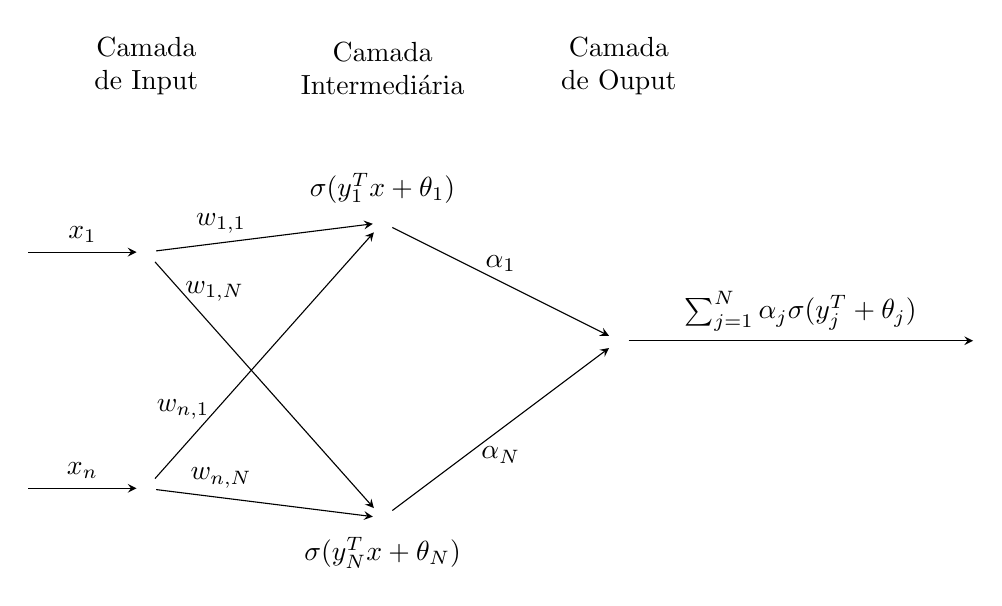
\begin{tikzpicture}[x=1.5cm, y=1.5cm, yshift=-1, >=stealth]

\foreach \m/\l [count=\y] in {1,missing,2}
  \node [every neuron/.try, neuron \m/.try] (input-\m) at (0,1.75-\y) {};

\foreach \m [count=\y] in {1,missing,2}
  \node [every neuron/.try, neuron \m/.try ] (hidden-\m) at (2,2.25-\y*1.25) {};

\foreach \m [count=\y] in {1}
  \node [every neuron/.try, neuron \m/.try ] (output-\m) at (4,1-\y) {};

\foreach \l [count=\i] in {1,n}
  \draw [<-] (input-\i) -- ++(-1,0)
    node [above, midway] {$x_\l$};

%% \foreach \l [count=\i] in {1,n}
%%   \node [above] at (hidden-\i.north) {$H_\l$};
\node [above] at (hidden-1.north) {\( \sigma (y_{ 1 }^{ T }x + \theta_{ 1 }) \)};
\node [below] at (hidden-2.south) {\( \sigma (y_{ N }^{ T }x + \theta_{ N }) \)};

\foreach \l [count=\i] in {1}
  \draw [->] (output-\i) -- ++(3,0)
    node [above, midway] {\( \sum_{ j=1 }^{ N } \alpha_{ j } \sigma (y_{ j }^{ T } + \theta_{ j }) \)};

%% \foreach \i in {1,...,2}
%%   \foreach \j in {1,...,2}
%%     \draw [->] (input-\i) -- (hidden-\j)
%%         node [above,pos=.2] {\( y_{ 1 }^{ (1) } \)};
\draw [->] (input-1) -- (hidden-1)
    node [above, pos=.3] {\( w_{ 1,1 } \)};
\draw [->] (input-2) -- (hidden-1)
    node [above, pos=.2, xshift=-2mm] {\( w_{ n,1 } \)};
\draw [->] (input-1) -- (hidden-2)
    node [above, pos=.2,xshift=2mm] {\( w_{ 1,N } \)};
\draw [->] (input-2) -- (hidden-2)
    node [above, pos=.3] {\( w_{ n,N } \)};

%% \foreach \i in {1,...,2}
%%   \foreach \j in {1}
%%     \draw [->] (hidden-\i) -- (output-\j);
\draw [->] (hidden-1) -- (output-1)
    node [above, midway] {\( \alpha_{ 1 } \)};
\draw [->] (hidden-2) -- (output-1)
    node [below, midway, yshift=-1mm] {\( \alpha_{ N } \)};

\foreach \l [count=\x from 0] in {de Input, Intermediária, de Ouput}
  \node [align=center, above] at (\x*2,2) {Camada \\ \l};

\end{tikzpicture}
    \end{center}
\end{frame}

\begin{frame}{Overview de Redes Neurais}{O que são redes neurais?}
    \vspace{2pt}
    A rede mostrada até o momento tem apenas uma camada oculta, mas redes neurais em geral têm várias.
    \begin{center}
        \includegraphics[width=.7\textwidth]{../figuras/multi-layer-neural-network.jpeg}
    \end{center}
\end{frame}

\begin{frame}{Overview de Redes Neurais}{Para que servem?}
    \vspace{2pt}
    Diversas aplicações:
    \begin{itemize}
        \item Classificação de imagens, incluindo reconhecimento facial;
        \item Predição de séries temporais;
        \item Análise de regressão;
        \item O algoritmo usado pela inteligência artificial \emph{AlphaGo} emprega redes neurais convolucionais (CNNs).
    \end{itemize}
\end{frame}

%%%%%%%%%%%%%%%%%%%%%%%%%%%%%%%%%%%%%%%%%%%%%%%%%%%%%%%%%%%
%%%%%%% The vital question: Faz sentido tudo isso? %%%%%%%%
%%%%%%%%%%%%%%%%%%%%%%%%%%%%%%%%%%%%%%%%%%%%%%%%%%%%%%%%%%%

\end{document}

